\begin{margintable}[6cm] %MARGIN TABLE
\begin{center}
\caption{A table of values of $e^{-x^2}$.} 
\label{T:5-6-EG3} 
\begin{tabular}{cc}
$x_i$ & $e^{-x_i^2}$ \\ \hline
$0$ & $1$\\
$0.25$ & $0.939$ \\
$0.5$ & $0.779$ \\
$0.75$ & $0.570$ \\
$1$ & $0.368$\\
\end{tabular}
\end{center}
\end{margintable}


\begin{example} \label{eg:5.6.3} % EXAMPLE
Approximate $\ds\int_0^1 e^{-x^2}\ dx$ using Simpson's Rule and $4$ equally spaced subintervals.

\solution We begin by making a table of values as we have in the past, as shown in Table~\ref{T:5-6-EG3}.

Simpson's Rule states that $$\int_0^1e^{-x^2}\ dx \approx \frac{0.25}{3}\Big[1+4(0.939)+2(0.779)+4(0.570) + 0.368\Big] = 0.7468\overline{3}.$$

Recall in Example \ref{eg:5.6.2} we stated that the correct answer, accurate to $4$ places after the decimal, was $0.7468$. Our approximation with Simpson's Rule, with $4$ subintervals, is better than our approximation with the Trapezoidal Rule using $5$.

Figure~\ref{F:5-6-EG3} shows $f(x) = e^{-x^2}$ along with its approximating parabolas, demonstrating how good our approximation is. The approximating curves are nearly indistinguishable from the actual function.
\end{example}

\begin{marginfigure}[-1cm] %MARGIN FIGURE
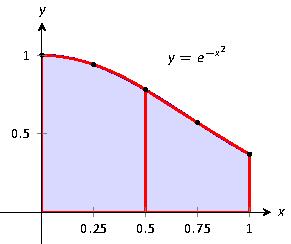
\includegraphics{figures/fignum5b} %Example 136 APEX
\caption{Approximating $\int_0^1 e^{-x^2}\ dx$ using Simpson's Rule.}
\label{F:5-6-EG3}
\end{marginfigure}